\documentclass[10pt]{article}
\usepackage[english]{babel}
\usepackage[latin1]{inputenc}
\usepackage{subfigure}
\usepackage{epsfig}
\usepackage{amsmath,amssymb}
\parindent 0mm
\textwidth 16cm
\textheight 23cm
\oddsidemargin 0cm
\evensidemargin 0cm
\topmargin -10mm
\newcommand{\vect}[1]{{\bf{#1}}}
\newcommand{\svect}[1]{\boldsymbol{#1}}
\newcommand{\matr}[1]{\boldsymbol{#1}}


\begin{document}
\pagestyle{empty}
\begin{Large}
\begin{bf} 
T-61.5130 Machine Learning and Neural Networks\\ 
\end{bf}
\end{Large}
Karhunen, Hao Tele\\  
\\
\begin{large}
\begin{bf}
Exercise 11, 09.12.2011
\end{bf}
\end{large}
\begin{enumerate}

\item In this problem we consider the optimized form of the learning
vector quantization algorithm developed by
Kohonen. We wish to arrange for the effects of the corrections to the
Voronoi vectors, made at different times, to have equal influence when
referring to the end of the learning period. \begin{enumerate}
   \item First, show that
   \begin{equation*}
   \mathbf{w}_c(n+1)=\mathbf{w}_c(n)+\alpha_n[\mathbf{x}_i-\mathbf{w}_c(n)]
   \end{equation*}
   and
   \begin{equation*}
   \mathbf{w}_c(n+1)=\mathbf{w}_c(n)-\alpha_n[\mathbf{x}_i-\mathbf{w}_c(n)]
   \end{equation*}
   may be integrated into a single equation, as follows:
   \begin{equation*}
   \mathbf{w}_c(n+1)=(1-s_n\alpha_n)\mathbf{w}_c(n)+s_n\alpha_n\mathbf{x}(n).
   \end{equation*}
   In the above equations, $\mathbf{w}_c$ is the Voronoi
   vector closest to the input vector $\mathbf{x}_i$, $0<\alpha_n<1$ is a
   learning constant, and $s_n$ is a sign function depending on the
   classification result of the $n$th input vector $\mathbf{x}(n)$:
   $s_n=+1$ if classification is correct, otherwise  $s_n=-1$.

   \item Hence, show that the optimization criterion described at the
   beginning of the problem is satisfied if
   \begin{equation*}
   \alpha_n=(1-s_n\alpha_n)\alpha_{n-1}
   \end{equation*}
   which yields the optimized value of the learning constant
   $\alpha_n$ as
   \begin{equation*}
   \alpha_n^{\text{opt}}=\frac{\alpha_{n-1}^{\text{opt}}}{1+s_n\alpha_{n-1}^{\text{opt}}}.
   \end{equation*}
\end{enumerate}

\vspace{2mm}

%\item Show that a recurrent MPL having two hidden layers can be represented by the state-space model
%\begin{eqnarray*}
%  \mathbf{x}(n+1) & = & \mathbf{f}(\mathbf{x}(n),\mathbf{u}(n))\\
%  \mathbf{y}(n) & = & \mathbf{g}(\mathbf{x}(n),\mathbf{u}(n))\; ,
%\end{eqnarray*}
%where $\mathbf{u}$ is the input, $\mathbf{y}$ is the output,
%$\mathbf{x}$ is the state, and $\mathbf{f}$ and $\mathbf{g}$ are
%vector-valued nonlinear functions.

\vspace{2mm}

\item Using the LMS-algorithm, formulate a learning algorithm for the
  focused neuronal filter.

\vspace{2mm}

\item How would you design a tapped delay line for a focused time
  lagged feedforward network?

\vspace{2mm}

\item Discuss how the temporal back-propagation algorithm may be used for the
  training of a distributed TLFN for single-step prediction.



%\item Is it possible to transform any state-space model into a NARX
%  model (in which the output is fed back to the inputs through a delay
%  line)? How about vice versa?
%
%\vspace{2mm}
%
%\item Construct an example of a network that is observable and of a
%  network that is not. Do the same after replacing observability with
%  controllability.
%
\vspace{2mm}

\item Write out the state-space model for the recurrent network shown in the
  figure below.

\hspace{2cm}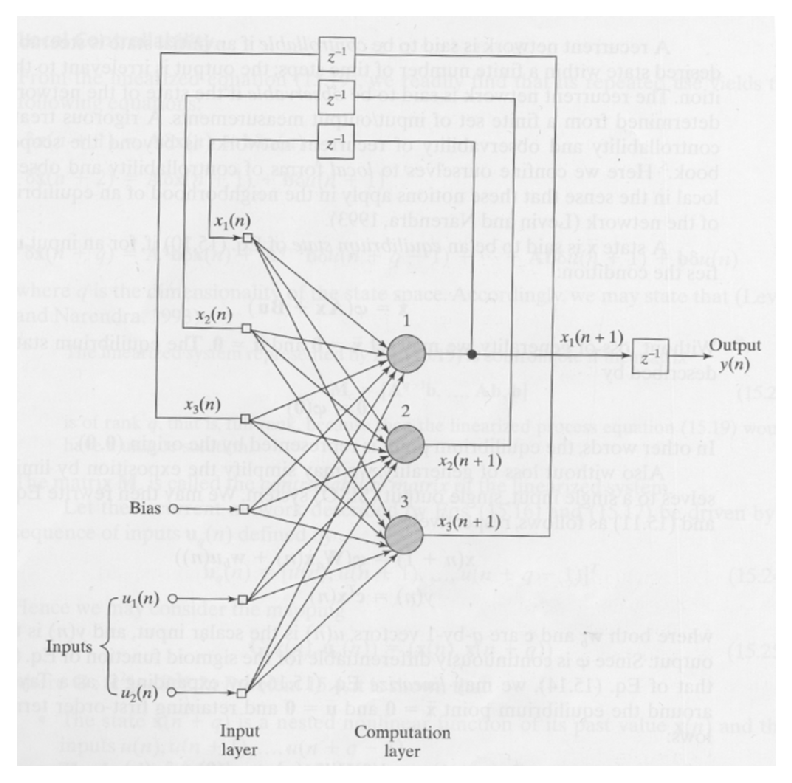
\includegraphics[width=11cm]{l12k9.eps}


\end{enumerate}
\end{document}             % End of document.
